% ------------------------------------------------------------------------------------
% # Chapter: SimWrapper
% ------------------------------------------------------------------------------------

Having confirmed the utility and capabilities of a fully browser-based
data visualization approach for three individual project portals, we
then set out to generalize the method. An entirely generic data
visualization platform is inherently more difficult than a project
portal, as every researcher investigates widely disparate questions and
will be focusing on completely different outputs. Where one researcher
may be using MATSim to predict future dynamic-response shared taxi
vehicle flows, another is doing emergency-response evacuation planning,
or emissions reduction through increased transit ridership efforts. The
tool needs to be extremely flexible.

% \begin{figure}
%   \centering
% 	\begin{minipage}{.75\textwidth}
% 		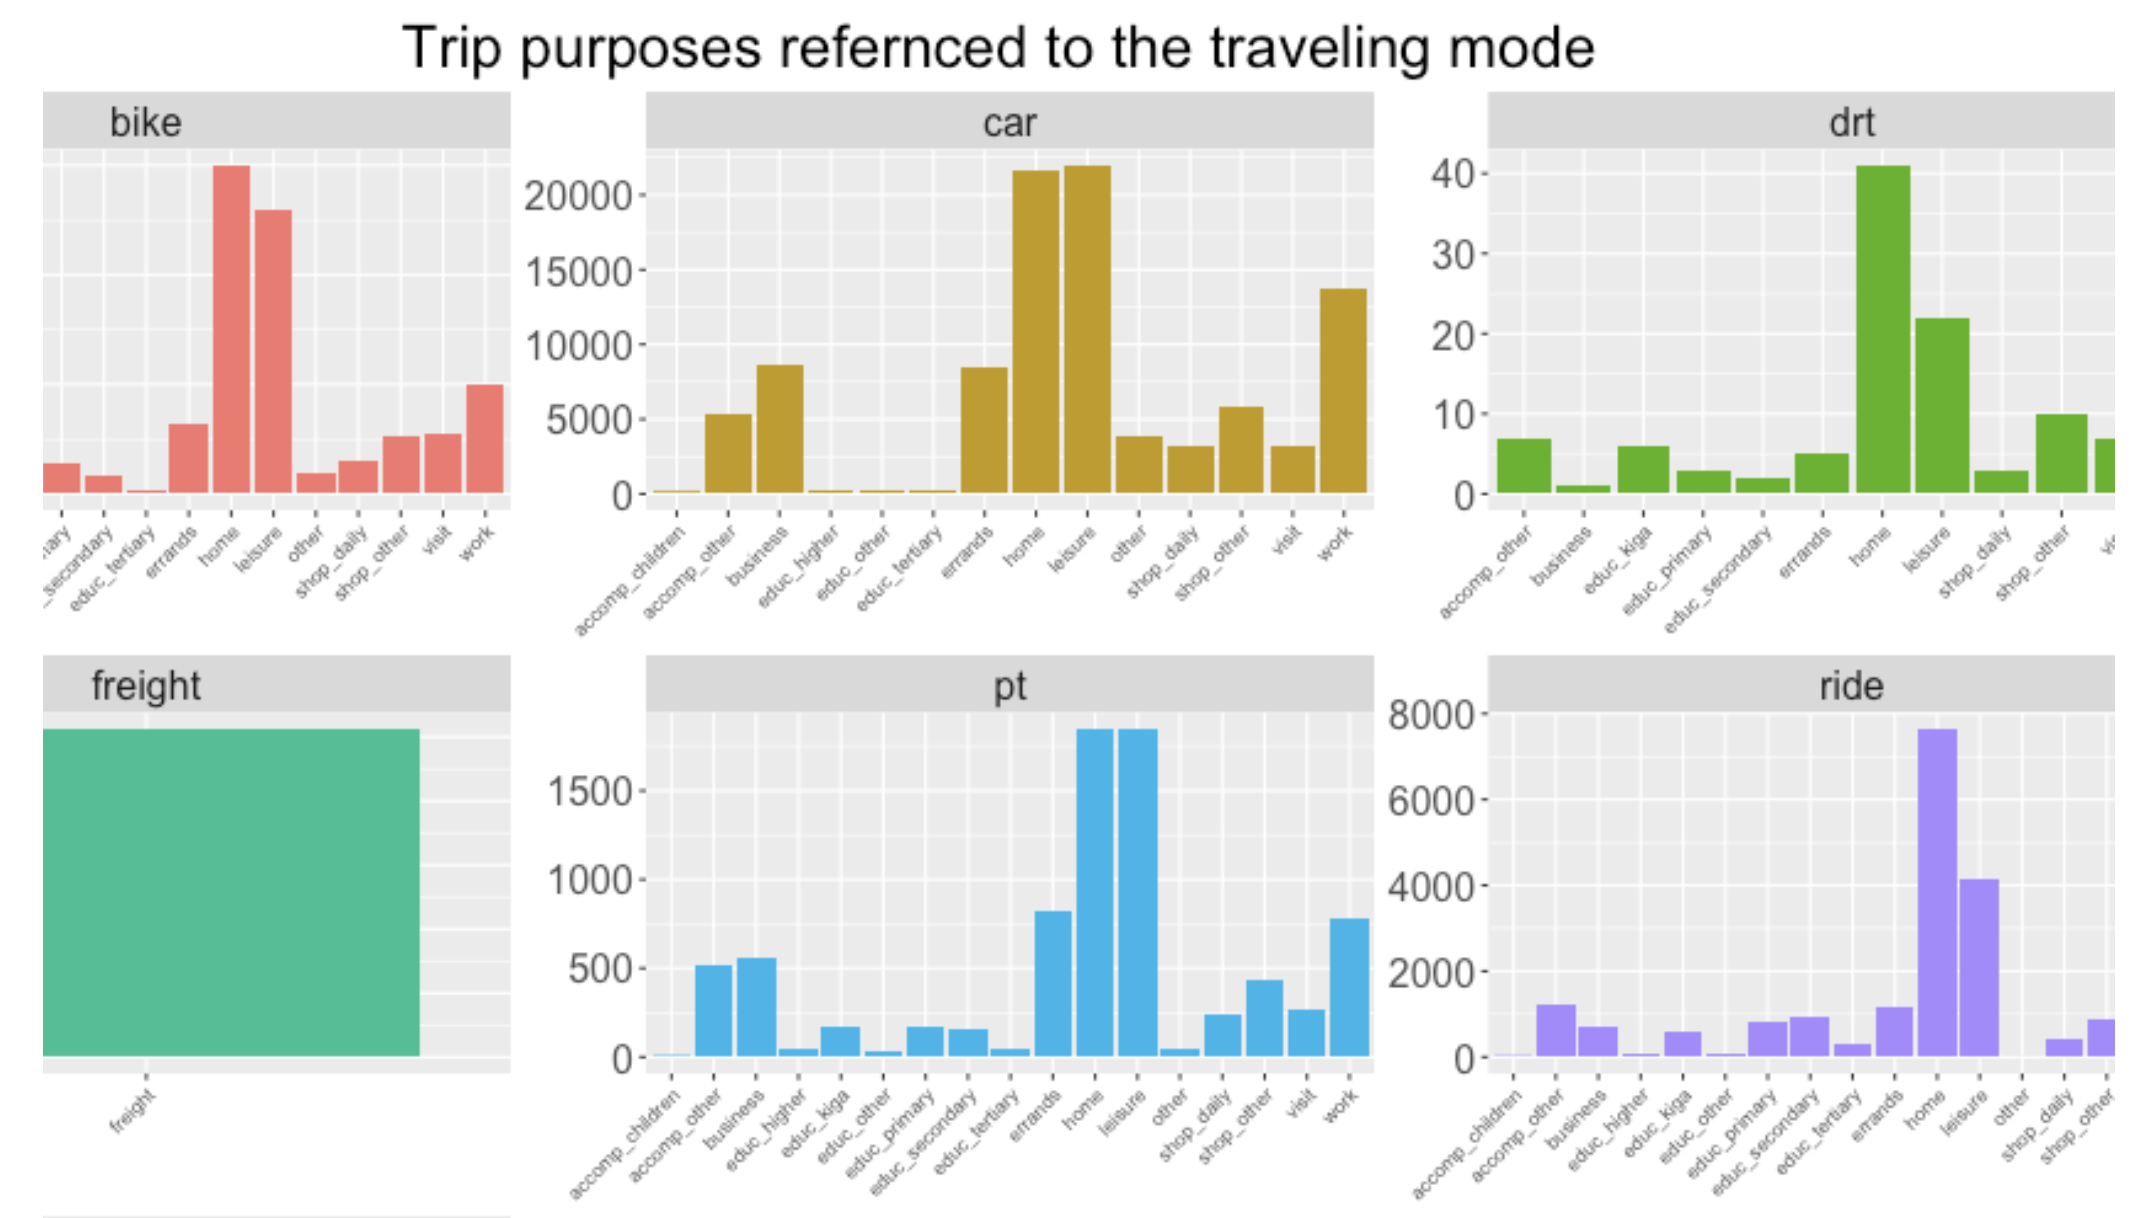
\includegraphics[width=\textwidth]{chapters/06-simwrapper/images/charts.png.pdf}
% 		\caption{CHart: stuff.}
% 		\label{fig:chartychart}
% 	\end{minipage}
% \end{figure}

This chapter describes \textbf{SimWrapper}, an open-source web-based
data visualization platform we developed with the goal that it be useful
for anyone working with MATSim outputs or even outputs from other
data-intensive microsimulation models.

% ------------------------------------------------------------------------------------
% ## SimWrapper in a Nutshell
% ------------------------------------------------------------------------------------

\hypertarget{overview-simwrapper-in-a-nutshell}{%
\section{Overview: SimWrapper, in a
nutshell}\label{overview-simwrapper-in-a-nutshell}}

Many design questions were already settled in the aforementioned
research YY.

SimWrapper, in a nutshell:

\begin{itemize}
\item
  \begin{enumerate}
  \def\labelenumi{(\arabic{enumi})}
  \item
    is a static website that runs client-side javascript in the form of
    a ``single page application'', a common approach in current web
    development that is compatible with all modern web browsers;
  \end{enumerate}
\item
  \begin{enumerate}
  \def\labelenumi{(\arabic{enumi})}
  \setcounter{enumi}{1}
  \item
    supports network-based file storage for public- and/or
    group-accessible shared data files (model runs), but has no other
    back-end server requirements and can run completely locally if no
    network file storage is available or needed;
  \end{enumerate}
\item
  \begin{enumerate}
  \def\labelenumi{(\arabic{enumi})}
  \setcounter{enumi}{2}
  \item
    allows the user to navigate through their local filesystem or shared
    network storage of model runs to view results that are saved in a
    specific folder, rather than a database-centric approach. This
    matches the design of MATSim and other simulation models which
    produce collections of output files by default;
  \end{enumerate}
\item
  \begin{enumerate}
  \def\labelenumi{(\arabic{enumi})}
  \setcounter{enumi}{3}
  \item
    provides a collection of data visualization archetypes that are each
    appropriate for displaying a certain type of data, for example
    various statistical chart types (bars, lines, area, pie), geographic
    data viewers supporting road and transit network link data, area
    aggregation (``choropleth'' and ``spider'') maps, XY coordinate
    plots, and many more;
  \end{enumerate}
\item
  \begin{enumerate}
  \def\labelenumi{(\arabic{enumi})}
  \setcounter{enumi}{4}
  \item
    can combine all of these disparate components into cohesive
    dashboards that the user can lay out in a flexible manner, using
    small declarative configuration files. These configurations can be
    applied across multiple projects or simulation runs;
  \end{enumerate}
\item
  \begin{enumerate}
  \def\labelenumi{(\arabic{enumi})}
  \setcounter{enumi}{5}
  \item
    is GDPR (General Data Protection Requirement) compliant by default,
    due to the complete lack of any user tracking, data uploads,
    servers, advertising, or any other privacy-compromising misfeatures.
    SimWrapper is not a product for sale; it is an open research
    platform, and can therefore forego these modern nuisances.
  \end{enumerate}
\end{itemize}

The following sections explore the design of SimWrapper in more detail.

\textbf{YY diagram of design}

% ------------------------------------------------------------------------------------
% ## Reusing existing components from previous projects
% ------------------------------------------------------------------------------------

\hypertarget{reuse-of-existing-framework-and-components}{%
\section{Reuse of existing framework and
components}\label{reuse-of-existing-framework-and-components}}

The starting point for SimWrapper was the PAVE project website described
in section YY. This ``single page application'' approach involves
selecting a curated set of javascript infrastructure libraries for
common needs, and then writing bespoke code for our specific use case
and the ``glue'' between the components.

Our experience with PAVE led us to select existing Javascript libraries
for the following:

\begin{itemize}
\item
  User interface interaction: the ``Vue'' framework YY is the primary
  glue that links the page layout with user interactions such as mouse
  clicks, running code when user-initiated events occur
\item
  Data loading: Most MATSim outputs are either tabular text files in CSV
  format, or compressed XML files with explicit schemas. The Papaparse
  and Fast-XML-Parser libraries handle loading these two data formats
\item
  Charting: the PAVE site included statistical charts such as bar, line,
  pie, and scatter plots, and used the Plotly javascript library. Plotly
  is very easy to use but not as feature-rich as some other choices; see
  below YY for updated capabilities
\item
  Geographic data on maps: our initial efforts using the Mapbox
  javascript library led us to the more performant Deck.gl collection of
  map-based visualizations.
\item
  Animation: Three.js is a very flexible 3D animation library that is
  used for PAVE vehicle animation visualizations.
\end{itemize}

All of these libraries share compatible open-source licenses, and are
included in SimWrapper under the terms of those licenses.

% ------------------------------------------------------------------------------------
% ## Modifications needed for a generic tool
% ------------------------------------------------------------------------------------

\hypertarget{modifications-necessary}{%
\section{Modifications necessary}\label{modifications-necessary}}

Direct user feedback, described in detail in section YY, allowed us to
map out a set of changes and improvements for the generic tool. In
summary, changes were needed in the following categories:

\begin{itemize}
\item
  Performance. The network link viewer in particular was slow to load
  datasets for large simulations. This was not a problem for PAVE or
  AVÖV because the study areas were less populated.
\item
  Flexibility. Each of the data visualization components needed to be
  made much more flexible. For example, the PAVE link viewer assumed
  that input data was specified by time period, whereas a generic tool
  needs to depict any sort of data.
\item
  Output traversal. While PAVE had a hard-coded set of alternatives that
  could be browsed in a simple manner, a generic tool needs some sort of
  model run traversal capability; a way to browse the hierarchical file
  storage available.
\item
  Stability and resilience. The PAVE site included almost no error
  message reporting or helpful debugging infrastructure, because expert
  analysts carefully crafted the inputs for each alternative. A generic
  tool needs to be tolerant of user mistakes and helpful in guiding the
  user when inputs are lost or malformed.
\item
  Better defaults plus configurability. We do not intend to replicate a
  full-featured desktop application, of which there are many in the
  Geographic Information System (GIS) realm. Rather, users expressed a
  desire for a set of clear, curated defaults that have some
  configurability. For much more advanced configuration, a
  professionally-developed package such as QGis is likely more
  appropriate.
\end{itemize}

\hypertarget{audience}{%
\subsubsection{Audience}\label{audience}}

The PAVE website was intended to be public-facing: both agency staff and
actual members of the public could navigate the site. It presented a
small set of YY six alternatives, depicting the same visualizations for
each alternative.

SimWrapper could be public facing, but is predominantly used in its
current form by researchers and professional analysts at public
agencies.

YY

% ------------------------------------------------------------------------------------
% ## Accessing files via a Web Browser
% ------------------------------------------------------------------------------------

\hypertarget{accessing-files-through-a-web-browser}{%
\section{Accessing files through a web
browser}\label{accessing-files-through-a-web-browser}}

The use case of file storage via departmental file server is
well-explored and very functional, as expressed in the project websites
for AVÖV, PAVE, and COVID-Sim.

A key difference between the earlier project websites and SimWrapper is
the need to ``meet the users where they are'' -- in other words, we
cannot rely on there being a departmental file server with a public API
endpoint serving data files. One of the primary feedback elements from
the initial MatHub implementation described in chapter YY was that it
was too onerous to upload model run outputs to a second server system
before being able to view or analyze anything. In addition to being
wasteful of space (and MATSim outputs can be gigabytes in size!), it is
time-consuming.

For regular users in the middle of their research workflow, something
else is needed. Most of our internal users run simulations either on
their personal laptop/desktop machines, or on the university compute
cluster, which has extensive attached storage but no public-facing
access via the web. Furthermore, these runs are often not intended to be
immediately publicized.

Thus we explore several avenues for enabling users to view their
outputs, described here.

% ------------------------------------------------------------------------------------
% ### How SimWrapper access files via HTTP
% ------------------------------------------------------------------------------------

\hypertarget{how-simwrapper-access-files-via-http}{%
\subsection{How SimWrapper access files via
HTTP}\label{how-simwrapper-access-files-via-http}}

SimWrapper is designed to allow browsing of files from
administrator-defined HTTP URLs, which represent the root of the file
storage for that project. For example, the PAVE project datasets are all
stored on the VSP public file server at the URL

\url{https://svn.vsp.tu-berlin.de/repos/public-svn/matsim/scenarios/countries/de/berlin/projects/pave/website/}

That URL is the defined ``root'' of the project; all of the project
dashboard configurations, model outputs, and processed data files exist
in various subfolders below that location. The PAVE website at
https://vsp.berlin/pave is set up to read files from that base URL. (But
refer to section YY for a discussion of CORS configuration, which is
necessary to allow one website to read the files stored on another.

SimWrapper elevates this to allow multiple configured root filesystems;
the public VSP file server is one such root, but others can also be
configured and are displayed on the home page of SimWrapper. Each root
is expected to provide HTTP directory access to this storage: SimWrapper
needs to be able to \emph{view directory listings} and \emph{retrieve
file contents}. SimWrapper never writes any files anywhere; it is
read-only.

% ------------------------------------------------------------------------------------
% ### Local files
% ------------------------------------------------------------------------------------

\hypertarget{local-files-on-a-personal-laptopdesktop}{%
\subsection{Local files on a personal
laptop/desktop}\label{local-files-on-a-personal-laptopdesktop}}

This design presents a problem for local files: By design, all web
browsers explicitly forbid file-system access from any websites by
default. This default is certainly a good default; no one wants any
random website to start sniffing around their home directory.

But in our case this is not any random website: we \emph{want}
SimWrapper to see the files in some of our local folders. How can this
be accomplished?.

After several explorations including raw HTML files opened directly,
arcane experimental browser flags (always vendor specific!), and other
less fruitful avenues, the one method that consistently works for all
browsers is as follows: for browsing local files on a machine, first
start up a small helper application which is itself a simple HTTP
server. This tiny server responds to HTTP requests and delivers the
directory contents requested. The server listens on ``localhost'',
i.e.~your own computer, generally on port 8000. So the full URL is
\url{http://localhost:8000/}.

Once this is set up and running, this HTTP endpoint can be accessed in
SimWrapper just like any other external file storage. SimWrapper knows
be default to look for files at URL \url{http://localhost:8000}.

As part of this research we wrote a very small Python library which
provides this server. Any machine with Python 3.x installed can run
\texttt{pip\ install\ simwrapper} to install this mini file server, and
then run it by navigating to their data folder and running the command
\texttt{simwrapper\ serve}. That includes all of the server components
and configuration needed to server files to SimWrapper.

Some configuration notes:

\begin{itemize}
\item
  The local HTTP server will only serve the files from inside the
  working directory in which it is started, including any subfolders. No
  other folders on the user's machine are exposed.
\item
  The computer's operating machine has default firewall and router rules
  that will generally prohibit any outside access from other computers
  on the LAN or the Internet. This can be modified; see YY
\item
  Some configuration details for the server that are important for our
  use case: we must enable access from websites at different URLs using
  ``CORS'' configuration headers; see YY
\item
  Some browsers (Safari, and now recent builds of Chrome) sometimes
  block access to localhost sites or http sites (vs.~https sites), see
  discussion at YY
\item
  Every language framework already includes some sort of ``Tiny HTTP
  Server'' library for just these types of uses: in Python it is in the
  \texttt{http.server} library, in Java there is the Jibble
  SimpleWebServer. Our \texttt{simwrapper} python tool leverages the
  existing Python infrastructure.
\item
  We also wrote a java version, published as
  \texttt{mini-file-server.jar} for users who are more comfortable
  running Java-based software than Python.
\end{itemize}

The Python tool including source and user documentation is currently
available at \url{https://pypi.org/project/simwrapper/}.

The Java tool is currently available at
\url{https://github.com/simwrapper/mini-file-server}

\hypertarget{data-security-and-privacy}{%
\subsubsection{Data security and
privacy}\label{data-security-and-privacy}}

With this setup, the SimWrapper site itself is loaded from the Internet,
but once loaded, the user's data never leaves their computer. SimWrapper
is an entirely client-based system with absolutely no upstream server.
The javascript runs in the users' browser, accessing files available on
localhost only -- also on the user's own computer. Nothing leaves the
browser. If there are privacy or confidentiality issues with model
outputs, SimWrapper can still be used for analysis in this ``localhost''
mode.

% ------------------------------------------------------------------------------------
% ### Files on Compute Cluster servers
% ------------------------------------------------------------------------------------

\hypertarget{files-residing-on-the-university-compute-cluster-accessed-via-ssh}{%
\subsection{Files residing on the university compute cluster, accessed
via
SSH}\label{files-residing-on-the-university-compute-cluster-accessed-via-ssh}}

This local-http-server paradigm can be extended to access files on any
remote university computer cluster using the SSH (``secure shell'')
protocol.

SSH is usually the protocol (and command) used to log into remote
systems. There is a parallel command which allows ``mounting'' the
remote file system using the SSH protocol. The remote files are mapped
to a folder on the user's system; once mounted, the user can browse the
files inside that folder as if they were local files (but generally more
slowly, depending on network throughput conditions).

\begin{itemize}
\item
  Linux users can install the command \texttt{sshfs} to add this
  capability;

  \begin{itemize}
  \item
    once installed, a command similar to
    \texttt{sshfs\ username@cluster.math.tu-berlin.de:/net/myfiles\ cluster}
    will mount the remote folder \texttt{/net/myfiles} to my local
    folder \texttt{cluster}. You would change the username, URL, and
    folder names to match your situation.
  \item
    \texttt{sudo\ umount\ cluster} or similar to unmount.
  \end{itemize}
\item
  YY MacOS is similar to Linux but requires installing the sshfs fuse
  driver first
\item
  YY Windows users have many options for FUSE-based sshfs support, this
  repo is nice one \url{https://github.com/billziss-gh/sshfs-win}
\end{itemize}

% ------------------------------------------------------------------------------------
% ### Files on other machines: simwrapper here
% ------------------------------------------------------------------------------------

\hypertarget{files-residing-on-another-machine-on-the-local-lan-network}{%
\subsection{Files residing on another machine on the local LAN
network}\label{files-residing-on-another-machine-on-the-local-lan-network}}

A challenging use case presented by users is one or more central
``modeling server'' machines on the local LAN, where most runs are
performed and which contain the simulation outputs.

The aforementioned localhost-based HTTP server does not work in this
situation, because a user sitting at their computer, opening the
Internet-based SimWrapper website, trying to read files served via
localhost on the modeling server, will always be blocked by browser
security measures. After many hours trying to find a way to sneak around
these restrictions, we accepted that this security measure is working as
designed, and we need a different approach.

The reason this approach is blocked is because the SimWrapper website is
hosted on a secure ``HTTPS'' server, while the localhost files must be
served without encryption using HTTP. Setting up an encryption
certificate is difficult because internal LAN machines don't typically
have world-findable DNS entries. This combination of secure and insecure
content is blocked by all browsers.

A workaround is to serve the files and the site from the same file
server, instead of using the Internet-based SimWrapper that is hosted at
vsp.berlin. We are already asking users to run a small file server to
access their local files, thus extending that file server to also serve
the necessary javascript and HTML is a natural extension.

And this is what we have done: a special mode is added to the
\texttt{simwrapper} python tool named \texttt{simwrapper\ here}. Now the
little server will serve both the file contents of the folder in which
it is started, \emph{and} the SimWrapper website itself.

The user runs \texttt{simwrapper\ here} on the file server instead of
\texttt{simwrapper\ serve}, \emph{noting the full URL printed in the
console}, and then on their personal computer browses to that URL
instead of to vsp.berlin/simwrapper. In this manner, the site and any
local files stored on that server are made available, together.

This also implies that SimWrapper can be used completely offline once it
is installed.

% ------------------------------------------------------------------------------------
% ### Special case: Google Chrome
% ------------------------------------------------------------------------------------

\hypertarget{special-case-chrome-and-the-file-system-access-api}{%
\subsection{Special case: Chrome and the ``File System Access
API''}\label{special-case-chrome-and-the-file-system-access-api}}

Google Chrome and a subset of other browsers based on the Chromium
codebase implement an experimental API known as ``File System Access
API''. This is not part of the official Web specification, and it may
never be adopted by other browser vendors.

But for users running Google Chrome, this experimental API provides
another avenue for accessing local files, one which completely
eliminates the need for the local file server approaches above.

This is considered ``progressive enhancement,'' or in other words,
adding features to the website when the browser is identified as
supporting them.

On Chrome, users will see an additional element on the main page of
SimWrapper, a button allowing them to grant access to local files. The
browser will open a standard folder-picking dialog followed by a warning
that granting this permission will allow the SimWrapper site to view the
files in that folder. Et Voíla, that is exactly what we need.

Once permission is granted, local files are immediately visible without
any additional configuration. This permission can be revoked and may be
re-requested every time the browser restarts.

YY show browser grant access dialog

% ------------------------------------------------------------------------------------
% ## Converting purpose-built vizes into Generic Data Viewers
% ------------------------------------------------------------------------------------

\hypertarget{converting-purpose-built-visualizations-into-generic-data-viewers}{%
\section{Converting purpose-built visualizations into generic data
viewers}\label{converting-purpose-built-visualizations-into-generic-data-viewers}}

The underlying infrastructure -- the build system, the user interaction
libraries, and the choice of off-the-shelf components -- was more or
less complete after the PAVE, AVÖV, and COVID-Sim projects were
operational. But the specific views needed a great deal of retooling to
make them useful in a generic manner.

This section describes some of the most challenging aspects of this
process of genericizing SimWrapper.

% ------------------------------------------------------------------------------------
% ### Link Viewer
% ------------------------------------------------------------------------------------

\hypertarget{link-viewer}{%
\subsection{Link viewer}\label{link-viewer}}

The link viewer was originally scoped to display link volumes only, such
as a typical ``bandwidth plot'' commonly used in travel modeling. Even
for PAVE this was short-sighted, as the project team quickly found other
uses for the viewer such as link-based emissions.

Two critical updates made for SimWrapper are (1) the removal of the
assumption that the data inputs will always have time period data in the
columns, plus a summary ``grand total'' column; and (2) that colors and
widths must be configurable, preferably separately.

These changes are now part of SimWrapper -- see YY for a typical plot.

YY show a bandwidth plot

User testing shows that a great deal more is still necessary to meet
user expectations. Data filters and configurable hovers are two of the
most-requested enhancements.

YY user testing

% ------------------------------------------------------------------------------------
% ### XY Data Plots
% ------------------------------------------------------------------------------------

\hypertarget{xy-hexagon-plots}{%
\subsection{XY Hexagon plots}\label{xy-hexagon-plots}}

Much data is not link-based, even for transport simulations. Activity locations, home locations, pickups and dropoffs for transit and taxi modes, all have geographic coordinates associated with them but are not necessarily attached to specific links.

A new visualization type, the ``XY Hexagons'' plot, depicts these types of data by aggregating them into user-definable hexagonal buckets. The number of points inside the hexagons corresponds to a color or height; this is user-configurable.

YY show XY Hexagon plot

The default MATSim output \texttt{output\_trips.csv} includes this type of data, and is automatically viewable without any configuration at all if it is present in a SimWrapper data folder.

% ------------------------------------------------------------------------------------
% ## Calculation Tables
% ------------------------------------------------------------------------------------

\hypertarget{calculation-tables}{%
\section{Calculation tables: providing top-line summary metrics}\label{calculation-tables}}

Early in the development of SimWrapper, user feedback identified the need for reporting basic summary statistics and generating common aggregate values from model runs. These top-level summaries provide the first indication of useful results, such as overall mode share, average travel times, total emissions, and so forth. In addition, these measures are an excellent way to "sanity-check" a model run; in other words, to identify any obvious glaring errors in those topline numbers when compared to previously-established norms.

The first element needed is a straightforward way for users to specify the inputs, outputs, and formatting of calculation tables, compatible with the file-based configuration approaches already in use for the graphical visualizations. A second challenge is to formulate a clear and accurate scheme for specifying the needed calculations, including statistical transformations of the inputs such as counts, sums, and so on. Finally, the tool must perform those calculations in memory and produce the display the results.

These three elements are explored in order.

% ------------------------------------------------------------------------------------
% ### Calculation Table Config: Inputs, Files, Outputs
% ------------------------------------------------------------------------------------

\hypertarget{calculation-tables-definition}{%
\subsection{Specifying calculation table files, inputs, and outputs }\label{calculation-tables-definition}}

The most robust way to generate and display a table of numbers is by having the user develop their own post-processing scripts which output a simple CSV with the summary values and labels that they need. For this approach, nothing special is needed; whatever data analysis pipelines the analyst is already using are sufficient. Especially for more complex post-processing needs, using a high-quality platform such as Python or R is the recommended path.

For more simple summaries, we develop a way to extract and minimally process typical MATSim data files including CSV and XML formats. This is based on experience with the hesitancy of some analysts in our department to write Python and R scripts (since they are far more familiar with Java programming). If all one needs is the sum of a column of values or the count of some event types, learning Python and debugging a Python script is perhaps overkill.

As the file-based YAML configuration paradigm for SimWrapper is at this point well-established, a new YAML configuration schema for table calculations is the most natural way to express these table definitions.

A new \texttt{table-*.yml} YAML schema containing four sections emerged from extensive iteration with users. The four required sections are:

\begin{itemize}

  \item \textbf{files}: The set of input file or files required for the table. These can be raw MATSim outputs or the results of any pre- or post-processing that has already occurred in the analyst data pipeline.

  \item \textbf{interactive input entries}: This is a list of end-user-editable entries that are visible on interactive web form. Some calculations benefit from having a variable input which the user can specify; imagine fuel cost per liter, or number of vehicles in a taxi fleet. Each of these entries can have a default value.

  \item \textbf{calculations}: An ordered list of mathematical calculations to be performed. Variables, data columns, and interactive elements specified above are combined in equations as needed. This is described in more detail below.

  \item \textbf{outputs}: The final table entries are specified with formatting and labels.

\end{itemize}

Three of the four sections --- \emph{files}, \emph{interactive entries}, and \emph{outputs} --- are trivially specified and do not require extensive exposition here: they are straightforward definitions of file names, titles, and formatting directives. These are well-documented in the YY documentation available on the SimWrapper Website (\cite{SimWrapperWebsite}).

The calculations are explored next.

% ------------------------------------------------------------------------------------
% ### Calculation Table DSL: Specifying the Equations
% ------------------------------------------------------------------------------------
\hypertarget{calculation-tables-dsl}{%
\subsection{Specifying calculations using a Domain-Specific Language}\label{calculation-tables-dsl}}

The final and most important piece of specifying calculations is devising the equation format to be used in the YAML configuration, which brings together the interactive value inputs, the required input files, data columns in those files (and any data manipulations thereon), and combines them all in understandable algebraic equations that can be solved by the tool.

This is more akin to a "domain-specific language" (DSL) YY ACRONYM than a configuration file.

\cite{Visser2008} defines a domain-specific language as follows, "A domain-specific language (DSL) is a high-level software implementation language that supports concepts and abstractions that are related to a particular (application) domain." Visser explains further that a DSL is in essence "the encapsulation of design and implementation knowledge from a particular application or technical domain. The commonalities of the domain are implemented directly in a conventional programming language or indirectly in code generation templates, while the variability is configurable by the application developer through some configuration interface."

This is precisely what the YAML calculation definitions set out to do: allow a user who is an expert in the dataset and the needed transformations for a particular metric, to define that in a manner that doesn't require them to write a data analysis script in a full-fledged programming language such as R or Python.

YY continue



% - Need a way to write equations
% - How to specify pieces of data from the inputs: files, columns, elements
% - transformations
% - filtering: two ways


% ------------------------------------------------------------------------------------
% ### Calculation Tables: Map/Reduce your way to an answer
% ------------------------------------------------------------------------------------
\hypertarget{calculation-tables-map-reduce}{%
\subsection{Calculating summary values via "map/reduce"}\label{calculation-tables-map-reduce}}

% - solve each equation, in top-down order
% - map/reduce columns of data using statistical functions
% - substitute values from out data
% - nerdamer does the math
% - final values can be displayed according to the formatting rules in 'output'


YY Show PAVE example run output with Sankey, numbers, etc

% ------------------------------------------------------------------------------------
% ## Dashboards
% ------------------------------------------------------------------------------------

\hypertarget{dashboards-combining-visualizations-to-support-decisionmaking}{%
\section{Dashboards: combining visualizations to support
decisionmaking}\label{dashboards-combining-visualizations-to-support-decisionmaking}}

A dashboard is a page laid out with multiple charts, plots, and
visualizations all together. The layout is defined in a YAML file that
contains the types of plots and their configuration parameters, all in
one place.

YY SHOW Dashboard \emph{Dashboards usually show several at-a-glance
summary metrics.}

In SimWrapper, a folder containing any number of \texttt{dashboard-*}
YAML files will display the dashboards in addition to the usual folder
browser view. When multiple dashboard YAML files exist, they will be
shown as multiple navigation tabs on the page.

\begin{itemize}
\item
  The layout consists of a set of named \textbf{rows}. The row name
  themselves are not shown anywhere, they are there to help organize the
  file.
\item
  Each \texttt{row} consists of a list of chart objects. By default, all
  objects in the row will be laid out horizontally from left to right,
  in equal widths. This can be configured.
\item
  Finally, each element in a row has specific properties that define the
  actual chart or visualization that will be displayed.

  \begin{itemize}
  \item
    \textbf{type} The chart or plot type, e.g.~\texttt{pie},
    \texttt{bar}, \texttt{flowmap}, etc. See the individual chart docs
    for all available plots.
  \item
    \textbf{title} The name of the plot
  \item
    \textbf{description} A brief description (optional)
  \item
    \textbf{width} One can set \emph{relative widths} by adding the
    \texttt{width:\ {[}number{]}} property. Charts have a default width
    of 1. Thus in a row with 3 charts, if the width of the first object
    is 2, then {[}2+1+1{]} means the first object fills 50\% of the row,
    and the remaining two objects fill 25\% each. (optional)
  \item
    \textbf{props} The set of configuration settings for this chart,
    such as the dataset to load, which columns to use, etc.
  \item
    \emph{The chart type determines the set of valid properties!}
  \end{itemize}
\end{itemize}

This system of defining dashboards in configuration has been used to
great effect in many internal studies

YY Show Düsseldorf (Hamburg?) ?

% ------------------------------------------------------------------------------------
% ## Project sites: Re-using and organizing outputs
% ------------------------------------------------------------------------------------

\hypertarget{project-traversal-and-organizing-outputs}{%
\section{Project traversal and organizing
outputs}\label{project-traversal-and-organizing-outputs}}

Project organization for MATSim is left up to the user: there is no
central database or general organizing principle which analysts must
adhere to. Thus different teams will find different ways to store their
data: by project, by date, by scenario type, etcetera. Some may use a
very flat structure with a defined naming scheme, while others will use
deeply nested folders to keep things tidy.

Because of this flexibility in MATSim, SimWrapper needs to be able to
handle deeply hierarchical storage as well as extremely large folders
full of runs.

There is much more room for improvement here, but the basic format of a
file and directory browser, which allows the user to ``drill down'' into
subfolders, will be part of any solution.

% ------------------------------------------------------------------------------------
% ### Calculation Table DSL: The Calculation Engline
% ------------------------------------------------------------------------------------


\hypertarget{project-level-configuration}{%
\subsection{Project-level
configuration}\label{project-level-configuration}}

Users often expressed interest in setting up standardized output
summaries in the form of dashboards, specific link- or xy-data
comparison plots, etc., and to use those for every model run for that
project.

This is addressed by having a \texttt{simwrapper} folder in or above the
output-data folders. The simwrapper folder contains any common
configuration files, whether they be dashboard layouts, individual
visualization parameters, or table calculation definitions. See YY for
more details on the configuration of individual components.

% ------------------------------------------------------------------------------------
% ## User Feedback and Iteration
% ------------------------------------------------------------------------------------

\hypertarget{user-feedback-and-iteration}{%
\section{User feedback and
iteration}\label{simwrapper-user-feedback}}

% ------------------------------------------------------------------------------------
% ## Limitations
% ------------------------------------------------------------------------------------

\hypertarget{limitations}{%
\section{Limitations}\label{simwrapper-limitations}}

% ------------------------------------------------------------------------------------
% ## Discussion
% ------------------------------------------------------------------------------------

\hypertarget{discussion}{%
\section{Discussion}\label{simwrapper-discussion}}
